\chapter{Development of Medication Tracking Application}
\label{Kap3}

%talking about platforms in general, to get a common understanding 
\section{Used platforms and technologies} \label{platforms}

\subsection{Native Development with NativeScript} 

There exist several ways to create a mobile application. But the challenge is to develop a consistent solution for the existing systems, like e.g. Android or iOS.
To face the challenge of developing both an Android and iOS application, one has to think of the usage of web development technologies, like for example HTML5, CSS and Javascript. These technologies provide the advantage of using the access to browser/internet  connection.

\subsubsection{NativeScript Sidekick}

\begin{figure}
\centering
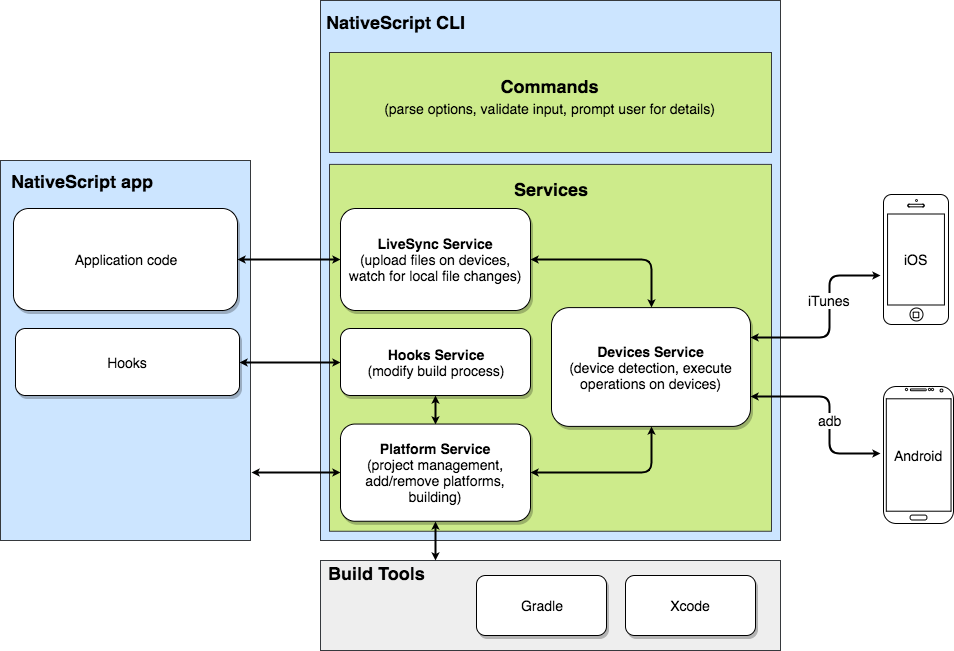
\includegraphics[width=\textwidth]{nativescript_functionality} The architecture of NativeScript Applications
\caption{\label{fig:nsarchitecture}The adopted from \cite{nsarchitecture}} 
\end{figure}



editor for writing simultaneously apps at one moment (both for Android and iOS devices)

\subsection{NoSQL Technology: MongoDB} \label{nosql}

\subsubsection{Characteristics of NoSQL Databases}

\subsubsection{Reasons and Advantages of MongoDB}

strong consistency and atomicity
secondary indexes 
ad hoc queries
querying/indexing/updating similar to relative databases (like SQL/Microsoft Access)

\subsection{Impinj RFID Lector and Antenna}

\subsubsection{General Information}

\subsubsection{Examples}

%
% talking about application, more details
%
\section{Application development}

\subsection{Challenges during development}

Mongodb integration within nativescript application 
--> with Node JS package installer 
but synchronization with data from Mongodb was difficult

\subsection{Progress of development}

\subsubsection{User Scenario}

\subsubsection{Software Architecture}

\begin{figure}
\centering
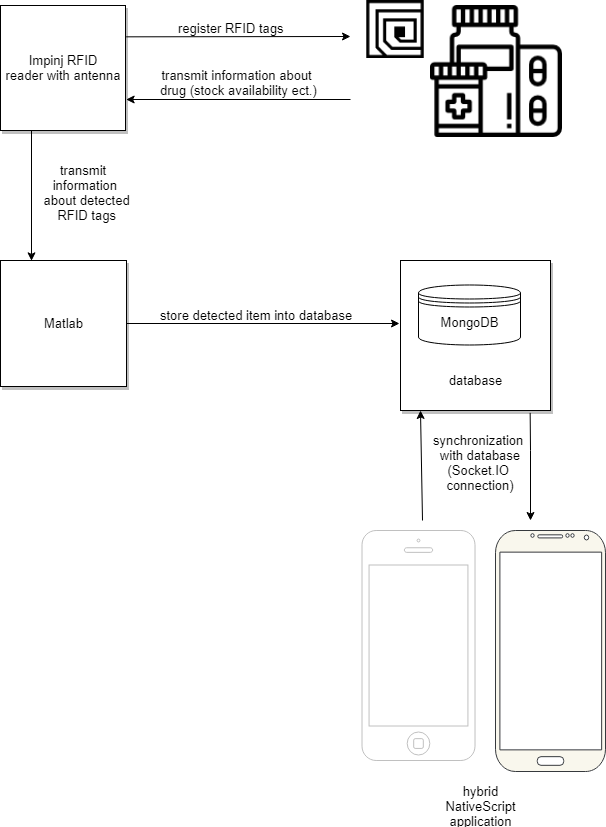
\includegraphics[width=\textwidth]{app_architecture} The developed system architecture of the mobile RFID application
\caption{\label{fig:apparchitecture}} 
\end{figure}

picture of general software architecture: 
2 antennas, 1 lector (RFID Impinj), Database (MongoDB), GUI: Android and  iOS Application 

\subsection{Possibilities of extension}

Henrici \cite[p.121 ff.]{henrici} describes four alternative channels to authenticate and authorized the right tags and to prevent attacks on RFID applications. 
The first possibility of an alternative channel is to use written text to authenticate special operations, for instance on packaging. The master key can be printed on the interior of the product package and is proposed as key recovery mechanism.
Furthermore, optical barcodes can be used together with RFID to ensure identification of items. Especially barcodes attached to each item can be used for general identification of objects. Additionally, RFID tags might be used to assign items of high value.
A third possibility of using side channels is to use optical input, such as photodiodes attached to RFID tags. Each RFID tag can use flashes of light (also called optical channel) to transfer data.   
Lastly, a physical contact channel can also be used alternatively. Compared to smartcards, this methods defends against wireless sabotage or denial of service attacks.


















 
